\documentclass[conference]{IEEEtran}
\IEEEoverridecommandlockouts
% The preceding line is only needed to identify funding in the first footnote. If that is unneeded, please comment it out.
\usepackage{cite}
\usepackage{amsmath,amssymb,amsfonts}
\usepackage{algorithmic}
\usepackage{algorithm}
\usepackage{graphicx}
\usepackage{textcomp}
\usepackage{xcolor}
\usepackage{booktabs}
\usepackage{float}
\usepackage[hidelinks]{hyperref}
\usepackage{listings}
\usepackage{microtype}
\usepackage{xurl}
\usepackage{balance}
\usepackage{xcolor}

\lstset{
  basicstyle=\ttfamily\small,
  keywordstyle=\color{blue},
  commentstyle=\color{gray},
  frame=single,
  breaklines=true,
  numbers=left,
  numberstyle=\tiny
}

\def\BibTeX{{\rm B\kern-.05em{\sc i\kern-.025em b}\kern-.08em
    T\kern-.1667em\lower.7ex\hbox{E}\kern-.125emX}}
    
\begin{document}

\title{Object Re-Identification with Locality Sensitive Hashing\\
}


\author{
\begin{tabular}{ccc}
\begin{minipage}[t]{0.30\textwidth}\centering
{\large Dr. Jyothi S. Nayak}\\
\textit{Department of CSE}\\
\textit{B.M.S. College of Engineering}\\
Bengaluru, India\\
jyothinayak.cse@bmsce.ac.in
\end{minipage}
&
\begin{minipage}[t]{0.30\textwidth}\centering
{\large Sarthaka Mitra G.B}\\
\textit{Department of CSE}\\
\textit{B.M.S. College of Engineering}\\
Bengaluru, India\\
sarthakamitra.cs23@bmsce.ac.in 
\end{minipage}
&
\begin{minipage}[t]{0.30\textwidth}\centering
{\large Skanda Mahesh}\\
\textit{Department of CSE}\\
\textit{B.M.S. College of Engineering}\\
Bengaluru, India\\
skandamahesh.cs23@bmsce.ac.in
\end{minipage}
\end{tabular}

\\[2em]

\hspace{0.0\textwidth}
\begin{tabular}{cc}
\begin{minipage}[t]{0.30\textwidth}\centering
{\large Subramanya J}\\
\textit{Department of CSE}\\
\textit{B.M.S. College of Engineering}\\
Bengaluru, India\\
subramanyaj.cs23@bmsce.ac.in
\end{minipage}
\end{tabular}
}

\setlength{\emergencystretch}{1em}
\maketitle

\begin{abstract}
Object re-identification on modest camera nodes benefits from an explicit connection between the observed foreground region and the evidence used to retrieve it. This paper presents a classical pipeline that forms coherent object observations, extracts a masked 602-dimensional appearance descriptor, and retrieves candidate exemplars using random-hyperplane locality-sensitive hashing (LSH) followed by exact cosine scoring. A substantial core test, normalized size constraints, and temporal confirmation suppress isolated fragments before feature extraction. The descriptor combines regional color, multiscale texture, gradient structure, and channel statistics; mutable hash tables retain references to bounded identity exemplars. An evaluation separates controlled motion replay, held-out rendered crops, and clustered-vector search diagnostics. On a 10,000-vector diagnostic, eight 12-bit tables with radius-one probing reduce the candidate fraction to 2.63\% and achieve a 4.77-fold query speedup over exhaustive search. Controlled motion replay yields a confirmed-box F1 score of 0.9744 and mask intersection-over-union of 0.7405. The study establishes an inspectable implementation and a measurable efficiency envelope, while image-descriptor ablations identify the next improvements in illumination robustness and acceptance calibration.
\end{abstract}

\begin{IEEEkeywords}
object re-identification, foreground segmentation, handcrafted descriptor, locality-sensitive hashing, approximate nearest neighbors, reproducible evaluation
\end{IEEEkeywords}

\section{Introduction}
Re-identification associates observations of a physical object when continuous tracking is unavailable, for example after the object leaves one camera and appears in another. The difficulty begins before retrieval: a foreground fragment, an oversized bounding box, or background contamination can change the appearance vector substantially. An efficient index cannot recover identity information that was lost while forming the observation. A useful system must therefore explain both what it bounds and how that bounded evidence becomes a searchable representation.

Recent object and vehicle Re-ID methods use transformer representations, self-supervised learning, and domain adaptation to improve discrimination under viewpoint and illumination changes~\cite{transreid2021,git2023,ssbver2023,daynight2024,vehiclemae2025}. These developments motivate complementary investigation of a transparent classical pipeline whose parameters, memory organization, and failure modes can be inspected directly. Such a pipeline is useful for CPU-based prototypes and for studying the relationship between segmentation, representation, and candidate search without an additional training stage.

We present a stationary-camera pipeline that connects foreground support to temporal object formation, masked appearance embedding, binary signatures, and exact candidate verification. We use the term \emph{object} for a coherent foreground component satisfying geometric and temporal conditions. This operational definition supports the vehicle-oriented prototype and whole-object demonstrations; semantic classification is a separate task. Likewise, a hash collision supplies a retrieval candidate rather than a unique physical identity.

The main contributions are:
\begin{enumerate}
\item An integrated observation-formation procedure combining a substantial foreground core, tighter relative dimensions, component-specific masks, and temporal confirmation. Connected fine detail is retained around a valid core, while isolated thin fragments are screened out.
\item A 602-value masked descriptor, termed MVSV-G, with auditable dimensional accounting and block-normalized color, texture, structure, and statistical evidence.
\item A random hyperplane index with radius-one probing, explicit exemplar references, and exact cosine verification, together with a derivation of its collision and candidate admission probabilities.
\end{enumerate}
These contributions concern system integration, implementation detail, and evaluation of established components, and they do not claim a new background model or a new LSH family.

\section{Related Work}
\subsection{Classical Segmentation and Object Formation}
Adaptive Gaussian-mixture background subtraction provides a practical foreground estimate for stationary cameras~\cite{zivkovic2004,opencvmog2}. Its output is sensitive to shadows, small motion regions, and model adaptation. GrabCut refines foreground through graph-cut optimization~\cite{grabcut2004}, but its usefulness depends on initialization. Our pipeline uses component support and geometry before optional refinement, making the validity of the observed region explicit.

Temporal association adds evidence that a region persists as an object. ByteTrack demonstrates the importance of how detections are associated, including lower-confidence observations~\cite{bytetrack2022}. Our classical implementation instead gates foreground components and solves a one-to-one rectangular assignment~\cite{scipylsa}, using overlap, displacement, and size change. The distinction matters: our tracker consumes adaptive foreground regions rather than detections from a trained category model.

\subsection{Appearance Representations for Re-Identification}
TransReID models object appearance with transformer features~\cite{transreid2021}; GiT introduces graph interaction for vehicle representations~\cite{git2023}. Self-supervised vehicle Re-ID explores scalable representation learning~\cite{ssbver2023}, while CAViT incorporates contextual alignment for video objects~\cite{cavit2022}. Day--night adaptation~\cite{daynight2024}, VehicleMAE pre-training~\cite{vehiclemae2025}, and meta-learning across visual modalities~\cite{kamenou2023} address variations that a fixed appearance descriptor must also confront. Yi et al. organize the broader vehicle Re-ID literature and its challenges~\cite{yi2025survey}.

Our descriptor draws on established local binary patterns (LBP)~\cite{ojala2002} and gradient histograms~\cite{dalal2005}, combining them with masked regional statistics. ORB provides an optional local-verification channel in the application~\cite{orb2011}; the experiments here isolate the global visual descriptor and its index. The comparison with learned Re-ID is architectural: published recognition scores from different datasets are not used as numerical baselines for our generated inputs.

\subsection{Approximate Search and Dynamic Galleries}
Random-hyperplane hashing relates cosine similarity to binary collisions~\cite{charikar2002}. Multi-probe LSH expands the buckets visited per table to improve the space--recall tradeoff~\cite{lv2007multiprobe}. Our implementation uses a simple, reproducible ordering: the exact signature followed by every one-bit flip. It differs from the probability-ranked probing and distance family in the original multi-probe work.

Recent search research includes query-dependent bucketing in DB-LSH~\cite{dblsh2022}, billion-scale indexing in SPANN~\cite{spann2021}, and incremental updates in SPFresh~\cite{spfresh2023}. Window-filtered ANN emphasizes that eligibility restrictions change the search problem~\cite{windowann2024}. The NeurIPS ANN challenge assesses accuracy, performance, and hardware cost at much larger scales~\cite{annchallenge2022}. Together, these studies motivate reporting quality, time, and storage jointly rather than using candidate reduction alone as a speed claim.

\subsection{Evaluation Datasets and Remaining Design Questions}
VeRi provides a real surveillance benchmark for vehicle identities~\cite{veri2016}. Synthehicle supplies synthetic multi-camera vehicle tracking and segmentation data, including Re-ID baselines~\cite{synthehicle2023}. Synthetic data permits known labels and controlled variation; its relevance depends on the diversity and realism of the generator. Our small deterministic fixtures serve a narrower purpose: they isolate implementation behavior and index scaling. Neither VeRi nor Synthehicle is used as experimental data in this study.

Table~\ref{tab:literature} summarizes fifteen papers from 2021--2025. The resulting design questions are concrete: how should a coherent foreground region be admitted, which appearance blocks help under a specified perturbation, and when does a hash index outperform an optimized scan? The proposed methodology addresses these questions in a single inspectable implementation.

\section{Proposed Methodology}
\noindent\textit{Overview of the Proposed Framework:}
Let a frame be $I_t\in\mathbb{R}^{H\times W\times3}$. Each admitted observation contains a box $B=(x,y,w,h)$, component mask $M$, local track identifier $\ell$, quality $q$, and descriptor $\mathbf z$. Figure~\ref{fig:pipeline} shows the processing sequence. No camera identifier, timestamp, or ground-truth identity is appended to the visual descriptor.

\begin{figure}[t]
\centering
\fbox{\parbox{0.91\columnwidth}{\centering
Frame and adaptive foreground\\$\downarrow$\\
Component core, geometry, temporal confirmation\\$\downarrow$\\
Object-specific mask and quality admission\\$\downarrow$\\
Masked 602-value descriptor and normalization\\$\downarrow$\\
Binary signatures and nearby hash buckets\\$\downarrow$\\
Candidate union, exact cosine, object preview}}
\caption{The visual path from observation formation to retrieval. Hash tables contain exemplar references; full descriptors remain available for verification.}
\label{fig:pipeline}
\end{figure}

\subsection{Foreground Support and Coherent Components}
The default estimator is OpenCV MOG2~\cite{zivkovic2004,opencvmog2}. Its statistical interpretation at pixel $u$ is
\begin{equation}
\begin{aligned}
p(I_t(u)) &= \sum_{k=1}^{K_u}\pi_{k,t}(u)\,\mathcal{N}_{k,t}(I_t(u)),\\
\mathcal{N}_{k,t}(v) &= \mathcal{N}(v;\boldsymbol\mu_{k,t}(u),\Sigma_{k,t}(u)),\\
\sum_k\pi_{k,t}(u)&=1.
\end{aligned}
\end{equation}
OpenCV performs the mixture updates. Only mask value 255 is accepted as foreground; the shadow value 127 is kept separate. A four-second warmup initializes the background. A $3\times3$ elliptical opening and closing suppress small isolated noise, followed by filling enclosed holes of at most $0.001HW$ pixels.

For a connected component $C$, let $a_C=|C|$ and let $d(u,F^c)$ be the distance from pixel $u$ to the cleaned foreground complement. A substantial component satisfies
\begin{equation}
\begin{aligned}
a_C &\ge \max(9,\operatorname{round}(0.0008HW)),\\
\max_{u\in C}d(u,F^c)&\ge0.015\min(H,W).
\end{aligned}
\label{eq:core}
\end{equation}
The distance transform uses a zero border and OpenCV's five-mask approximation. Crucially, Eq.~\eqref{eq:core} tests the presence of a core and then retains its entire connected component. Thus, attached fingers can remain part of a palm-supported region while an isolated thin fragment fails admission. It does not broadly merge neighboring components or infer missing object parts.

\subsection{Normalized Bounding-Box Admission}
We define $r_y=\operatorname{clip}((y+h)/H,0,1)$. All of the following inequalities must hold:
\begin{equation}
\begin{aligned}
0.065&\le w/W\le0.80,\\
0.10&\le h/H\le0.85,\\
0.008(1+0.25r_y)&\le wh/(HW)\le0.40,\\
a_C/(HW)&\ge0.004,\\
a_C/(wh)&\ge0.30,\qquad 0.4\le w/h\le3.5.
\end{aligned}
\label{eq:gates}
\end{equation}
The width, height, and upper-area bounds act independently. The minimum area increases slightly toward the image bottom, while foreground occupancy rejects mostly empty rectangles. At $960\times540$, the minimum integer width and height are 63 and 54 pixels, respectively, and the support floor is 2,074 pixels. These normalized restrictions encode a target-size envelope that can be calibrated for the camera placement.

\subsection{Temporal Association and Observation Quality}
A track predicts its center using smoothed velocity. For track $i$ and component $j$, define center displacement $\delta_{ij}$ and scale change $\eta_{ij}$ as
\begin{equation}
\begin{aligned}
d_i&=\max(20,\sqrt{\widehat w_i^2+\widehat h_i^2}),\\
\delta_{ij}&=\|\operatorname{ctr}(\widehat B_i)-\operatorname{ctr}(B_j)\|_2/d_i,\\
\eta_{ij}&=\tfrac12\left(\left|\log\tfrac{\widehat w_i}{w_j}\right|
+\left|\log\tfrac{\widehat h_i}{h_j}\right|\right),\\
c_{ij}&=0.45(1-\operatorname{IoU}(\widehat B_i,B_j))\\
&\quad+0.40\delta_{ij}+0.15\eta_{ij}.
\end{aligned}
\end{equation}
Size ratios outside $[0.45,2.2]$ are rejected, as are pairs with IoU below 0.01 and $\delta_{ij}>0.85$. A rectangular linear assignment produces one-to-one associations~\cite{scipylsa}. Invalid fragments are removed before assignment so they cannot shrink an established track.

Measured velocity $\mathbf u_t$ updates the estimate and consistency:
\begin{equation}
\begin{aligned}
\mathbf v_t&=0.65\mathbf v_{t-1}+0.35\mathbf u_t,\\
e_t&=\|\mathbf u_t-\mathbf v_{t-1}\|_2\Delta t_m/d_i,\\
s_t&=0.7s_{t-1}+0.3\exp(-e_t).
\end{aligned}
\end{equation}
Here $\Delta t_m$ is time since the previous measured center. Confirmation requires six cumulative associated hits, $s_t\ge0.4$, and valid geometry. Tracks expire after more than 14 missed updates. A merged component containing two established track centers is withheld so the tracks can coast separately.

The crop is masked by its own component. Optional GrabCut~\cite{grabcut2004} uses a foreground core and background border, accepting refinement only when it retains at least 60\% of original foreground and its area is 0.55--1.6 times the original. Quality admission uses
\begin{equation}
\begin{aligned}
q_0&=0.20q_s+0.25q_l+0.20q_f+0.15q_v+0.20s_t,\\
q_s&=\min(1,\min(h_c,w_c)/90),\\
q_l&=\min(1,\operatorname{Var}_{M}(\nabla^2I)/180),\\
q_f&=\operatorname{clip}(1-|\phi-0.7|/0.7,0,1).
\end{aligned}
\label{eq:quality}
\end{equation}
Here $\phi=|M|/(h_cw_c)$ and $q_v$ is visible-box fraction. Severe clipping, low support, or insufficient size multiplies quality by 0.3; flagged occlusion multiplies it by 0.45. An observation is admitted at $q\ge0.42$. These terms are engineering scores, not probabilities of a correct identity.

\subsection{Masked Appearance Embedding}
The crop is aspect-preserving letterboxed to $128\times80$ pixels. Image and mask resizing use area and nearest-neighbor interpolation, respectively. Masked statistics exclude padding; texture and gradients use a $7\times7$ eroded interior, reverting to the original support if fewer than ten pixels remain. Table~\ref{tab:descriptor} accounts for every descriptor value.

\begin{table}[t]
\centering\small
\caption{MVSV-G dimensional decomposition.}
\label{tab:descriptor}
\begin{tabular}{lrp{0.55\columnwidth}}
\toprule Block & Values & Construction\\\midrule
Color & 180 & Regional histograms 156; Lab cell moments 24.\\
Texture & 54 & Three radii, each with 10 LBP and 8 variance bins.\\
Structure & 332 & Gradients 288; edges 10; silhouette and projections 34.\\
Statistics & 36 & Channel moments 18; covariances 15; global measures 3.\\\midrule
Total & 602 & Weighted, normalized concatenation.\\\bottomrule
\end{tabular}
\end{table}

\subsubsection{Color and joint statistics}
The whole crop and its upper and lower halves each contribute HSV histograms with 12/8/8 bins and Lab histograms with 8/8/8 bins. A $2\times2$ Lab partition contributes means and standard deviations. Histogram counts $n_b$ are transformed as
\begin{equation}
H_b=\sqrt{n_b/\max(1,\textstyle\sum_jn_j)}.
\end{equation}
This square-root frequency representation reduces domination by highly populated bins. For normalized HSV/Lab channel vector $\mathbf x_u\in\mathbb R^6$, covariance is
\begin{equation}
\widehat\Sigma=\frac{1}{n-1}\sum_{u\in M}
(\mathbf x_u-\overline{\mathbf x})(\mathbf x_u-\overline{\mathbf x})^\top.
\end{equation}
The 15 off-diagonal terms complement six channel means, standard deviations, and interquartile ranges. Mask occupancy, normalized aspect ratio, and mean gradient magnitude complete the statistics block.

\subsubsection{Texture and structure}
Eight circular neighbors at radius $R\in\{1,2,3\}$ define bits $b_p=\mathbf1[g_p\ge g_c]$. With circular transition count $U=\sum_{p=0}^{7}|b_p-b_{(p+1)\bmod8}|$, uniform rotation-invariant LBP~\cite{ojala2002} is
\begin{equation}
\operatorname{LBP}_{8,R}^{\mathrm{riu2}}=
\begin{cases}\sum_{p=0}^7b_p,&U\le2,\\9,&U>2.\end{cases}
\end{equation}
Each radius supplies ten LBP bins and eight log-variance bins. Sobel gradients form nine unsigned-orientation bins in each of $4\times8$ cells, inspired by HOG~\cite{dalal2005}. For cell $P$ and orientation bin $b$,
\begin{equation}
g_{P,b}=\sum_{u\in P\cap M_{\mathrm{int}}}
\|\nabla I(u)\|_2\,\mathbf1[\operatorname{bin}(\nabla I(u))=b].
\end{equation}
Each cell histogram is normalized. Nine Canny edge-orientation bins and edge density add ten values. A $6\times4$ silhouette and its four row and six column means add coarse occupancy structure. The local LBP rotation property does not imply full viewpoint invariance of the combined descriptor.

\subsubsection{Block normalization and cosine scoring}
Let $\mathcal U(\mathbf f)=\mathbf f/\max(\|\mathbf f\|_2,10^{-12})$. For blocks $C,T,G,S$ and weights $\boldsymbol\alpha=(1,0.65,0.70,0.40)$,
\begin{equation}
\begin{aligned}
\mathbf z&=\mathcal U\left(\mathop{\Vert}_{b\in\{C,T,G,S\}}
\alpha_b\mathcal U(\mathbf f_b)\right),\\
\mathbf z&\in\mathbb R^{602},\qquad s(\mathbf z,\mathbf z')=\mathbf z^\top\mathbf z'.
\end{aligned}
\label{eq:embedding}
\end{equation}
The symbol $\Vert$ denotes concatenation. When all blocks are nonzero,
\begin{equation}
s(\mathbf z,\mathbf z')=
\frac{\sum_b\alpha_b^2\mathcal U(\mathbf f_b)^\top\mathcal U(\mathbf f'_b)}
{\sum_b\alpha_b^2}.
\end{equation}
Thus weights influence cosine through their squares, while independent normalization prevents block length alone from determining influence. A descriptor-profile checksum records the feature version and weights for compatibility.

\subsection{Hash Generation and Table Organization}
For table $l$ and bit $j$, draw independent $\mathbf r_{lj}\sim\mathcal N(\mathbf0,I_{602})$ with a recorded random seed. The signature is
\begin{equation}
\begin{aligned}
h_{lj}(\mathbf z)&=\mathbf1[\mathbf r_{lj}^\top\mathbf z\ge0],\\
H_l(\mathbf z)&=\sum_{j=0}^{b-1}2^jh_{lj}(\mathbf z).
\end{aligned}
\end{equation}
The default $L=8$ tables and $b=12$ bits produce eight integers in $[0,4095]$. Planes and descriptors use float32, and bit zero is least significant. Similar vectors tend to share signatures, but many distinct objects can collide.

For a fixed unit-vector pair with angle $\theta$, a single random-hyperplane bit agrees with probability $p=1-\theta/\pi$~\cite{charikar2002}. Independence gives
\begin{equation}
\begin{aligned}
\theta&=\arccos(\operatorname{clip}(\mathbf z^\top\mathbf z',-1,1)),\\
q_0&=p^b,\qquad q_1=p^b+b(1-p)p^{b-1},\\
P_r&=1-(1-q_r)^L,\qquad r\in\{0,1\}.
\end{aligned}
\label{eq:probability}
\end{equation}
Here $q_1$ allows zero or one differing bit within a table, and $P_r$ is admission by at least one table. These probabilities describe random index construction for a fixed pair, not the probability that two observations show the same physical object.

Each dictionary maps an integer signature to a set of exemplar keys:
\begin{equation}
\begin{aligned}
T_l[a]&=\{k:H_l(\mathbf z_k)=a\},\\
R[k]&=(H_1(\mathbf z_k),\ldots,H_L(\mathbf z_k)).
\end{aligned}
\end{equation}
The reverse map $R$ supports removal without scanning all buckets. Updating a key first removes its old references, then inserts its new signature into each table. Empty buckets are deleted. Full descriptors remain in the gallery for exact scoring; hash tables store references to them.

The live gallery retains up to eight exemplars per identity. A near duplicate with cosine at least 0.985 replaces an older exemplar when quality improves. When retention is required, selection starts with the highest-quality item and then favors quality and diversity:
\begin{equation}
e^*=\arg\max_{e\in\mathcal P}
\left[0.55q_e+0.45\left(1-\max_{a\in\mathcal S}\mathbf z_e^\top\mathbf z_a\right)\right].
\end{equation}
Here $\mathcal S$ is the selected set and $\mathcal P$ the remaining pool. This bounds exemplars per identity; the fixed-gallery benchmark evaluates the retrieval primitive separately from online retention.

\subsection{Multi-Probe Retrieval and Exact Verification}
For an eligible-gallery set $E_q$, define the per-table probe signatures
\begin{equation}
\begin{aligned}
\mathcal A_l(q)&=\{H_l(\mathbf z_q)\}\\
&\quad\cup\{H_l(\mathbf z_q)\oplus2^j:0\le j<b\},\\
\mathcal K_q&=E_q\cap\bigcup_{l=1}^{L}\ \bigcup_{a\in\mathcal A_l(q)}T_l[a],\\
\widehat k&=\arg\max_{k\in\mathcal K_q}\mathbf z_q^\top\mathbf z_k.
\end{aligned}
\label{eq:retrieve}
\end{equation}
The XOR operation flips one bit. Candidate keys are deduplicated, then compared using the original normalized vectors. Empty candidate sets produce an abstention without an exhaustive fallback. The benchmark excludes self-samples and can exclude every same-camera gallery observation for cross-camera evaluation. The monitor pairs observed and reference crops with retrieval evidence so a user can inspect what a returned identifier represents.

\begin{algorithm}[t]
\caption{Visual observation and indexed retrieval}
\label{alg:pipeline}
\begin{algorithmic}[1]
\REQUIRE Frame $I_t$, track state, gallery, tables $T_l$
\STATE Estimate foreground and separate shadow support
\STATE Clean components; apply core and size tests
\STATE Associate admissible components with track predictions
\FOR{each currently confirmed track due for observation}
\STATE Form component-specific crop and mask
\STATE Compute quality using Eq.~\eqref{eq:quality}
\IF{$q\ge0.42$}
\STATE Extract normalized descriptor (Eq.~\eqref{eq:embedding})
\STATE Compute signatures and collect $\mathcal K_q$
\STATE Rank candidates by exact cosine (Eq.~\eqref{eq:retrieve})
\STATE Retain evidence and the observation preview
\STATE Update retained exemplar references when admitted
\ENDIF
\ENDFOR
\end{algorithmic}
\end{algorithm}

\subsection{Hyperparameter Selection}
Table~\ref{tab:parameters} records the principal settings. They were held fixed during each evaluation rather than optimized on its test queries. The tightened box envelope is an engineering revision; comparison with the earlier envelope checks its effect on the same motion sequence. The main retrieval configuration uses seed 17 operationally, while experiments repeat plane construction with seeds 17, 29, and 43. Index sensitivity also covers longer signatures, additional tables, and exact-bucket-only probing.

\begin{table}[t]
\centering\small
\caption{Principal fixed settings in the visual evaluation.}
\label{tab:parameters}
\begin{tabular}{p{0.57\columnwidth}p{0.32\columnwidth}}
\toprule Setting & Value\\\midrule
MOG2 history / variance threshold & 500 / 24\\
Background warmup & 4 s\\
Opening and closing kernel & $3\times3$ ellipse\\
Minimum core radius & $0.015\min(H,W)$\\
Track confirmation / expiry & 6 hits / $>14$ misses\\
Consistency / quality floor & 0.40 / 0.42\\
Canonical crop / descriptor & $128\times80$ / 602\\
Default tables / bits / probe radius & 8 / 12 / 1\\
Maximum live exemplars per identity & 8\\
Optional GrabCut in replay & Disabled\\
Diagnostic acceptance threshold & Cosine $\ge0.82$\\\bottomrule
\end{tabular}
\end{table}

\subsection{Computational Complexity}
With fixed background-model and morphology settings, foreground processing scales with the $HW$ image pixels. For $n$ tracks and $m$ components, forming association costs takes $O(nm)$; dense assignment has a cubic worst-case bound in the larger dimension. Canonical feature extraction has fixed image support and descriptor dimension $D=602$.

Hash projection costs $O(LbD)$ per observation. Radius-one probing visits $L(b+1)$ buckets, or 104 by default. If $V_q$ is the number of bucket references visited, candidate collection and scoring cost
\begin{equation}
T_q=O\bigl(LbD+V_q+|\mathcal K_q|D\bigr).
\end{equation}
Bounded top-$k$ selection adds candidate-dependent selection work. Dense buckets can make $V_q$ large; no unconditional sublinear query bound follows. Exhaustive scoring costs $O(ND)$ but benefits from contiguous matrix operations. Storage consists of $ND$ vector values, $LbD$ plane values, and $LN$ key memberships, with Python dictionary/set overhead measured separately. This analysis predicts an empirical break-even region rather than universal LSH superiority.

\section{Experimental Results}
\subsection{Experimental Setup}
\subsubsection{Datasets and protocol}
All reported measurements were produced locally on an AMD Ryzen 9 7940HS processor with eight cores and sixteen logical processors, Windows 11, Python 3.14.3, NumPy 2.5.3, SciPy 1.18.1, and OpenCV 4.14.0.94. OpenCV and BLAS thread counts were pinned to one for the research suite~\cite{numpyglobal}. Cameras and remote nodes were not started for these measurements.

The evaluation has three complementary, explicitly generated input families:
\begin{enumerate}
\item \emph{Controlled motion replay:} 80 background-only warmup frames followed by 100 evaluated $640\times360$ frames at timestamps spaced by 0.05 s. Two moving vehicle-shaped drawings provide 200 ground-truth boxes and foreground masks; a narrow moving distractor is a labeled negative. The actual foreground, tracking, crop-quality, and descriptor code processes these frames.
\item \emph{Rendered appearance retrieval:} 64 identity-specific drawings supply three gallery variants each, giving 192 gallery descriptors. One held-out variant per identity and 16 unknown identities give 80 queries. Translation, gain, noise, and query blur vary the crops. These are two-dimensional appearance perturbations, not physical camera viewpoints.
\item \emph{Clustered-vector diagnostics:} normalized 602-dimensional Gaussian identity centers receive independent noise with standard deviation 0.018. Five gallery observations per identity produce galleries of 100, 1,000, 5,000, and 10,000 vectors. Each size has 100 independently generated queries. This isolates search behavior under a specified angular distribution.
\end{enumerate}
The fixed data seed is 2026. Each index is constructed with three plane seeds. Five untimed query warmups precede five timed repetitions per query, with interleaved randomized method order. Timing includes projection, bucket collection, eligibility filtering, exact candidate scoring, and bounded top-10 selection. Complete rankings for accuracy are computed outside the timer. The archive retains raw per-query repetitions, generated descriptor inputs, parameters, package versions, and source fingerprints. The reported run is \texttt{paper-local-20260914} under the project's experiment results.

\subsubsection{Evaluation metrics}
One-to-one box matching at IoU $\ge0.5$ supplies true positives (TP), false positives (FP), and false negatives (FN):
\begin{equation}
\begin{aligned}
\mathrm{Precision}&=\frac{\mathrm{TP}}{\mathrm{TP}+\mathrm{FP}},\quad
\mathrm{Recall}=\frac{\mathrm{TP}}{\mathrm{TP}+\mathrm{FN}},\\
F_1&=\frac{2\mathrm{TP}}{2\mathrm{TP}+\mathrm{FP}+\mathrm{FN}},\\
\mathrm{IoU}(A,B)&=\frac{|A\cap B|}{|A\cup B|},\quad
\mathrm{Dice}(A,B)=\frac{2|A\cap B|}{|A|+|B|}.
\end{aligned}
\end{equation}
Mask scores aggregate pixel counts across evaluated frames; mean box IoU uses matched pairs. Detection candidates and confirmed tracks are scored separately so confirmation delay remains visible.

For a query $q$, let $R_q$ be the number of eligible relevant gallery descriptors, $r_q(k)$ the relevance at candidate rank $k$, and $P_q(k)$ precision through that rank. Then
\begin{equation}
\begin{aligned}
\mathrm{AP}(q)&=\frac{1}{R_q}\sum_{k=1}^{|\mathcal K_q|}P_q(k)r_q(k),\\
\mathrm{mAP}&=\frac{1}{|Q^+|}\sum_{q\in Q^+}\mathrm{AP}(q).
\end{aligned}
\end{equation}
The denominator includes all eligible positives, including those missed by hashing. $Q^+$ contains queries with a relevant gallery observation; unknown queries are scored separately at the fixed acceptance threshold. Rank-1 measures correct identity at first rank. Exact-top-1 candidate recall instead asks whether the exhaustive nearest descriptor is retained in the candidate set; these are distinct measures.

We additionally report candidate fraction, index build time, estimated reachable index memory, and shared gallery-vector bytes. Query latency is summarized by the median of repetitions per query, then the query median per seed. Table~\ref{tab:search} averages these seed-level medians and seed-level speed ratios. Query bootstrap intervals in the JSON archive are conditional on a fixed dataset and seed; temporally adjacent frames are not treated as independent population samples.

\subsubsection{Baseline methods}
The primary comparator is vectorized exhaustive cosine search on the same normalized vectors, exclusions, and top-10 selection task. LSH settings are $(L,b,r)=(8,12,0),(8,12,1),(8,16,1),(16,12,1)$. Descriptor ablations zero one block at a time and renormalize, using exhaustive retrieval to isolate representation effects. The earlier box envelope is replayed on identical motion frames. No learned baseline is claimed to have been trained or evaluated.

\subsection{Quantitative Results}
Table~\ref{tab:vision} reports the controlled motion results. Candidate boxes achieve complete detection of the 200 labeled object instances. Confirmation reduces recall to 0.95 because two tracks each require five initial unconfirmed observations before the sixth hit. No matched-track identity switch occurs in this separated-motion sequence. Both earlier and tightened size gates produce the same scores on these target sizes, showing preservation of these accepted objects rather than an empirical precision gain over the older gates.

\begin{table}[t]
\centering\small
\caption{Controlled synthetic motion replay: 100 evaluated frames, 200 target boxes.}
\label{tab:vision}
\begin{tabular}{lrr}
\toprule Metric & Candidates & Confirmed tracks\\\midrule
TP / FP / FN & 200 / 0 / 0 & 190 / 0 / 10\\
Precision & 1.0000 & 1.0000\\
Recall & 1.0000 & 0.9500\\
F1 & 1.0000 & 0.9744\\
Mean matched-box IoU & 0.8438 & 0.8356\\\midrule
Foreground mask IoU & \multicolumn{2}{c}{0.7405}\\
Foreground mask Dice & \multicolumn{2}{c}{0.8509}\\
Matched-track switches & \multicolumn{2}{c}{0}\\
Admitted confirmed crops & \multicolumn{2}{c}{190 / 190}\\\bottomrule
\end{tabular}
\end{table}

\begin{table*}[t]
\centering\small
\caption{Default LSH versus exhaustive cosine search. Times are milliseconds; averages cover three index seeds. Generated-vector results measure index behavior, not field Re-ID accuracy.}
\label{tab:search}
\begin{tabular}{lrrrrrrr}
\toprule Input & $N$ & Scan ms & LSH ms & Speedup & Candidates & Exact-top-1 recall & LSH mAP\\\midrule
Clustered vectors & 100 & 0.0095 & 0.0441 & $0.22\times$ & 7.10\% & 96.67\% & 0.9573\\
Clustered vectors & 1,000 & 0.0356 & 0.0510 & $0.70\times$ & 3.00\% & 96.33\% & 0.9547\\
Clustered vectors & 5,000 & 0.2976 & 0.1033 & $2.88\times$ & 2.70\% & 96.67\% & 0.9487\\
Clustered vectors & 10,000 & 1.0805 & 0.2267 & $4.77\times$ & 2.63\% & 98.33\% & 0.9527\\
Rendered MVSV-G & 192 & 0.0130 & 0.0757 & $0.17\times$ & 84.24\% & 99.58\% & 0.5942\\\bottomrule
\end{tabular}
\end{table*}

The indexed search achieves a $2.88\times$ speedup at 5,000 vectors and $4.77\times$ at 10,000 vectors (Table~\ref{tab:search}). At the largest size, only 2.63\% of the gallery is scored and exact-top-1 candidate recall is 98.33\%. Rank-1 identity accuracy on these well-separated generated clusters is 1.0, whereas LSH mAP is 0.9527 because some relevant exemplars are omitted. Exhaustive mAP is 1.0 on this diagnostic. The speedup ranges from 4.74 to 4.79 across the three seeds, showing repeatability for this fixed distribution and machine.

The rendered descriptor gallery provides a different and useful regime. Exact search obtains rank-1 of 0.6406 and mAP of 0.5962; default LSH mAP is 0.5942. Here hashing preserves nearly all exact nearest candidates but visits 84.24\% of the gallery, leaving insufficient savings to offset lookup overhead. Table~\ref{tab:ablation} explains an associated representation effect: removing color increases mAP to 0.7087 on the held-out brightness-shifted drawings, whereas removing structure reduces it to 0.5063. This identifies photometric robustness as a productive refinement and confirms useful structural evidence in this controlled test.

\begin{table}[t]
\centering\small
\caption{Descriptor ablation on 64 known rendered queries using exhaustive search. The 16 unknown queries are evaluated separately.}
\label{tab:ablation}
\begin{tabular}{lrr}
\toprule Descriptor & Rank-1 & mAP\\\midrule
Full MVSV-G & 0.6406 & 0.5962\\
Without color & 0.7656 & 0.7087\\
Without texture & 0.6406 & 0.5963\\
Without structure & 0.5313 & 0.5063\\
Without statistics & 0.6406 & 0.5886\\\bottomrule
\end{tabular}
\end{table}

\subsection{Qualitative Analysis}
Figure~\ref{fig:qualitative} shows an actual frame from the controlled replay, its processed mask, and confirmed boxes. The thin distractor is removed while the two substantial components remain separate. The mask score is lower than the box score because agreement of enclosing rectangles does not imply identical silhouettes. Component-specific support makes this distinction observable at the crop boundary.

\begin{figure*}[t]
\centering
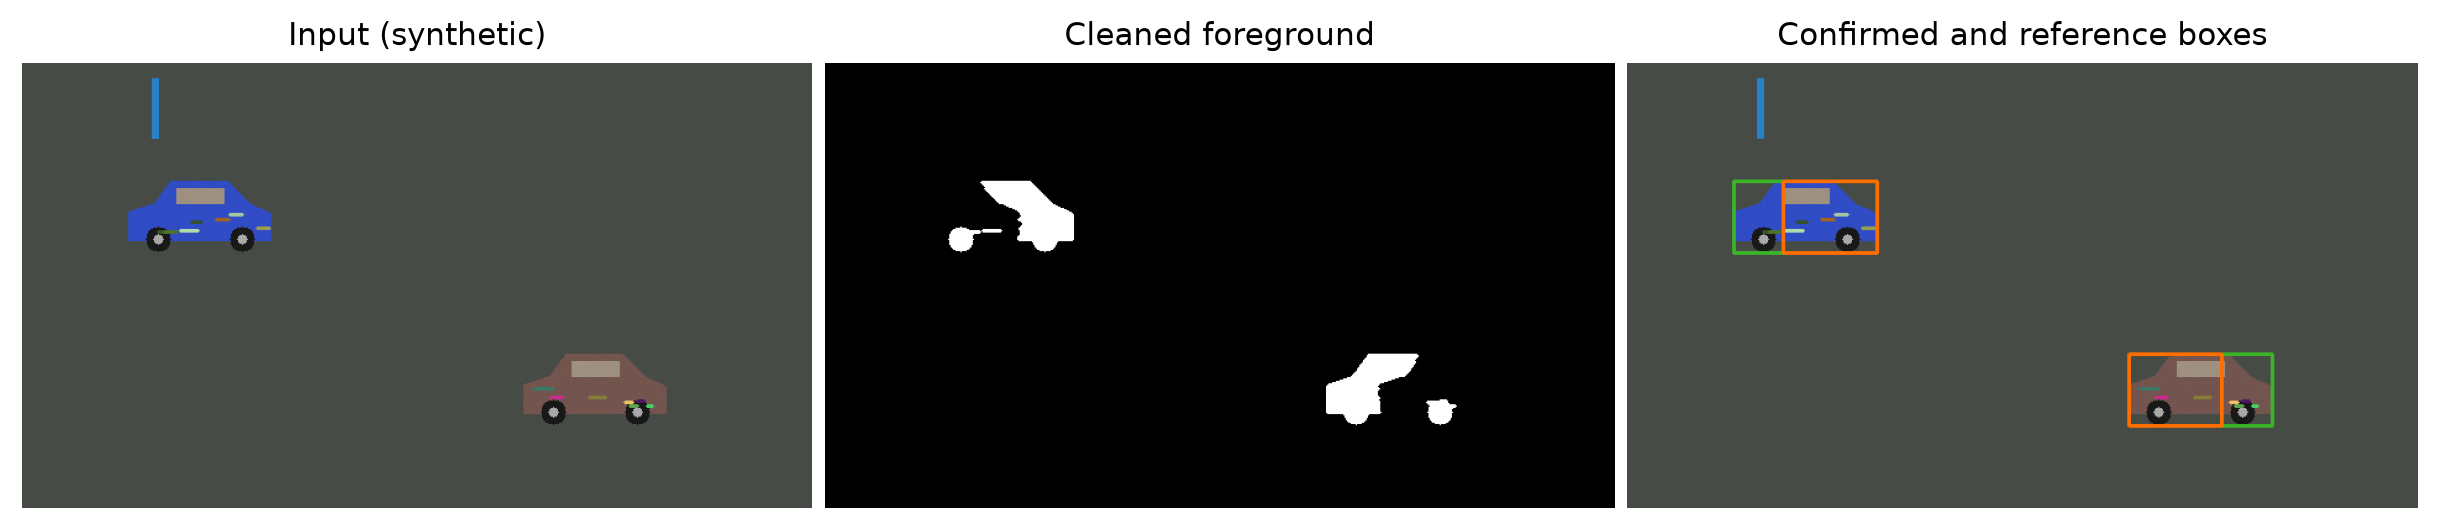
\includegraphics[width=\textwidth]{paper_figures/qualitative.png}
\caption{Controlled synthetic replay example generated by the same fixture and processed by the implemented foreground/tracker code. Left: input with a thin negative distractor. Center: cleaned foreground. Right: current confirmed boxes (orange), compared with ground-truth boxes (green). This is a diagnostic illustration, not captured LAN footage.}
\label{fig:qualitative}
\end{figure*}

The color ablation illustrates why adding feature blocks should be evaluated rather than presumed beneficial. Global appearance summaries remain concentrated in a limited portion of angular space on these drawings, which also produces high bucket occupancy. The monitor's paired thumbnails offer a practical way to inspect confusing matches during subsequent labeled camera runs, linking a retrieved identifier back to visible evidence.

\subsection{Runtime Performance}
The tightened-gate replay processes approximately 71.71 frames/s locally for foreground, tracking, crop-quality checks, and admitted descriptor extraction. This processing throughput excludes camera acquisition, asynchronous communication, and monitor display; it is therefore distinct from the application's 24-frame/s capture cap. At 10,000 vectors, the default index requires approximately 261.44 ms to build and 13.69 MB of estimated index memory, alongside 24.08 MB of shared float32 gallery vectors. These memory figures describe reachable Python/NumPy objects, not operating-system peak resident memory.

The small-gallery measurements are equally informative: exhaustive retrieval is faster at 100 and 1,000 diagnostic vectors and about 5.8 times faster for the 192 rendered descriptors. Figure~\ref{fig:latency} displays the measured scale transition. Consequently, the useful operating region depends on both gallery size and descriptor distribution. Candidate count and wall-clock timing must be considered together when selecting an index.

\begin{figure}[t]
\centering
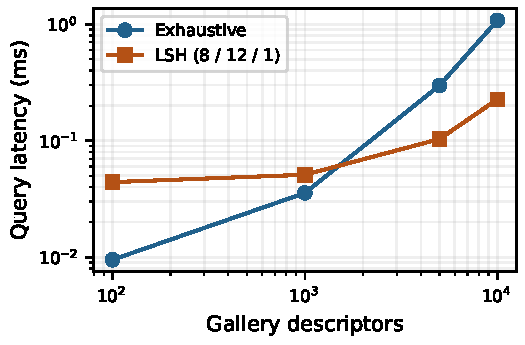
\includegraphics[width=\columnwidth]{paper_figures/search_latency.pdf}
\caption{Measured query latency for generated clustered vectors. The default index amortizes its lookup overhead at the larger tested gallery sizes. Each point averages three seed-level query medians.}
\label{fig:latency}
\end{figure}

\subsection{Discussion}
The results support an explicit and efficient visual retrieval path under controlled conditions. They also resolve several potential ambiguities. A valid region is a geometrically and temporally supported foreground observation, not a semantic category prediction. An embedding is a reproducible feature map; its similarity depends on the information retained by its blocks. A binary signature is a candidate-routing mechanism, with exact scoring required after collision. These distinctions make the method easier to audit and improve.

The principal experimental boundary is external validity. The motion drawings and perturbed crops are synthetic fixtures, and the Gaussian experiment is a search diagnostic. They exercise actual executable code and provide exact labels, but they do not establish cross-camera recognition accuracy on real footage. Synthetic evaluation has a clear precedent in Synthehicle~\cite{synthehicle2023}; our simpler generator offers much less scene and viewpoint diversity. Exhaustive-search baselines and joint quality--time--space reporting follow established ANN evaluation practice~\cite{lv2007multiprobe,annchallenge2022}. These precedents justify the evaluation questions and reporting method, not an equivalence between our inputs and published benchmarks.

One calibration result deserves explicit attention: all 16 unknown rendered queries are accepted at the diagnostic cosine threshold of 0.82 by both exhaustive search and default LSH. Thus the visual threshold alone does not provide reliable open-set rejection on these inputs. This result concerns the isolated cosine diagnostic, not an evaluated end-to-end live fusion decision. Together with the color ablation, it motivates independently calibrated thresholds, difficult negative examples, and photometric preprocessing. Crowded occlusion, camera movement, small distant targets, and stopped objects absorbed into the background also require broader evaluation.

To support that next step, every application run now writes \texttt{metrics\_live.json}, a unique run archive, and an observation-label template. Counts and measured processing times are available without labels. Identity precision, recall, and F1 are computed only after independent annotation, with resolution and annotation coverage reported. Undefined accuracy remains null rather than being inferred from generated IDs. Separate labeled frame and crop manifests allow the offline suite to evaluate real masks, boxes, and ranked retrieval. This provides a direct route from the present reproducible diagnostics to a field study with a held-out calibration/test split.

\section{Conclusion and Future Work}
This paper presents a transparent classical object Re-ID pipeline linking coherent foreground support, tighter bounding boxes, a masked 602-dimensional descriptor, mutable random-hyperplane tables, and exact candidate verification. The implementation makes the role of each stage explicit and preserves visual evidence alongside retrieved identities. Controlled replay demonstrates stable object formation on the tested sequence, while the 10,000-vector diagnostic demonstrates a 4.77-fold query speedup with 98.33\% exact-top-1 candidate recall. The contrast with concentrated image descriptors establishes a practical, distribution-dependent efficiency envelope.

Future work will prioritize independently labeled multi-camera footage, photometric robustness, validation-based open-set calibration, and a measured policy for choosing exhaustive or indexed search. The supplied experiment archive and live annotation exports make those extensions reproducible. The current contribution is a working, mathematically specified baseline whose measured strengths and targeted refinements provide a concrete foundation for further Re-ID research.

\IEEEtriggercmd{\balance}
\IEEEtriggeratref{10}
\begin{thebibliography}{00}

\bibitem{transreid2021}
S. He, H. Luo, P. Wang, F. Wang, H. Li, and W. Jiang,
``TransReID: Transformer-Based Object Re-Identification,''
in \textit{Proc. IEEE/CVF International Conference on Computer Vision (ICCV)},
pp. 15013--15022, Oct. 2021.


\bibitem{git2023}
F. Shen, Y. Xie, J. Zhu, X. Zhu, and H. Zeng,
``GiT: Graph Interactive Transformer for Vehicle Re-Identification,''
\textit{IEEE Transactions on Image Processing},
vol. 32, pp. 1039--1051, 2023, doi: 10.1109/TIP.2023.3238642.


\bibitem{ssbver2023}
P. Khorramshahi, V. Shenoy, and R. Chellappa,
``Robust and Scalable Vehicle Re-Identification via Self-Supervision,''
in \textit{Proc. IEEE/CVF Conference on Computer Vision and Pattern Recognition Workshops (CVPRW)},
pp. 5295--5304, 2023.


\bibitem{daynight2024}
H. Li, J. Chen, A. Zheng, Y. Wu, and Y. Luo,
``Day-Night Cross-domain Vehicle Re-identification,''
in \textit{Proc. IEEE/CVF Conference on Computer Vision and Pattern Recognition (CVPR)},
pp. 12626--12635, 2024.


\bibitem{vehiclemae2025}
Q. Wang, Z. Zhang, D. Wang, D. Gai, X. Xiong, J. Xu, and R. Zhou,
``VehicleMAE: View-asymmetry Mutual Learning for Vehicle Re-identification Pre-training via Masked AutoEncoders,''
in \textit{Proc. IEEE/CVF International Conference on Computer Vision (ICCV)},
pp. 4701--4711, Oct. 2025.


\bibitem{cavit2022}
J. Wu, L. He, W. Liu, Y. Yang, Z. Lei, T. Mei, and S. Z. Li,
``CAViT: Contextual Alignment Vision Transformer for Video Object Re-identification,''
in \textit{Proc. European Conference on Computer Vision (ECCV)}, 2022.


\bibitem{synthehicle2023}
F. Herzog, J. Chen, T. Teepe, J. Gilg, S. H\"ormann, and G. Rigoll,
``Synthehicle: Multi-Vehicle Multi-Camera Tracking in Virtual Cities,''
in \textit{Proc. IEEE/CVF Winter Conference on Applications of Computer Vision Workshops (WACVW)},
pp. 1--11, Jan. 2023.


\bibitem{kamenou2023}
E. Kamenou, J. Mart\'inez del Rinc\'on, P. Miller, and P. Devlin-Hill,
``A Meta-Learning Approach for Domain Generalisation Across Visual Modalities in Vehicle Re-Identification,''
in \textit{Proc. IEEE/CVF Conference on Computer Vision and Pattern Recognition Workshops (CVPRW)},
pp. 385--393, 2023.


\bibitem{yi2025survey}
X. Yi, Q. Wang, Q. Liu, Y. Rui, and B. Ran,
``Advances in vehicle re-identification techniques: A survey,''
\textit{Neurocomputing}, vol. 614, art. 128745, Jan. 2025.


\bibitem{dblsh2022}
Y. Tian, X. Zhao, and X. Zhou,
``DB-LSH: Locality-Sensitive Hashing with Query-based Dynamic Bucketing,''
in \textit{Proc. IEEE International Conference on Data Engineering (ICDE)},
pp. 2250--2262, 2022.


\bibitem{spann2021}
Q. Chen, B. Zhao, H. Wang, M. Li, C. Liu, Z. Li, M. Yang, and J. Wang,
``SPANN: Highly-efficient Billion-scale Approximate Nearest Neighbor Search,''
in \textit{Advances in Neural Information Processing Systems (NeurIPS)}, 2021.


\bibitem{annchallenge2022}
H. V. Simhadri \textit{et al.},
``Results of the NeurIPS'21 Challenge on Billion-Scale Approximate Nearest Neighbor Search,''
\textit{Proceedings of Machine Learning Research}, vol. 176, pp. 177--189, 2022.


\bibitem{windowann2024}
J. Engels, B. Landrum, S. Yu, L. Dhulipala, and J. Shun,
``Approximate Nearest Neighbor Search with Window Filters,''
in \textit{Proc. International Conference on Machine Learning (ICML)}, PMLR vol. 235, pp. 12469--12490, 2024.


\bibitem{spfresh2023}
Y. Xu \textit{et al.},
``SPFresh: Incremental In-Place Update for Billion-Scale Vector Search,''
in \textit{Proc. ACM Symposium on Operating Systems Principles (SOSP)}, 2023.


\bibitem{bytetrack2022}
Y. Zhang \textit{et al.},
``ByteTrack: Multi-Object Tracking by Associating Every Detection Box,''
in \textit{Proc. European Conference on Computer Vision (ECCV)}, pp. 1--21, 2022.


\bibitem{zivkovic2004}
Z. Zivkovic,
``Improved Adaptive Gaussian Mixture Model for Background Subtraction,''
in \textit{Proc. International Conference on Pattern Recognition (ICPR)}, 2004.


\bibitem{ojala2002}
T. Ojala, M. Pietik\"ainen, and T. M\"aenp\"a\"a,
``Multiresolution Gray-Scale and Rotation Invariant Texture Classification with Local Binary Patterns,''
\textit{IEEE Transactions on Pattern Analysis and Machine Intelligence},
vol. 24, no. 7, pp. 971--987, 2002, doi: 10.1109/TPAMI.2002.1017623.


\bibitem{dalal2005}
N. Dalal and B. Triggs,
``Histograms of Oriented Gradients for Human Detection,''
in \textit{Proc. IEEE Conference on Computer Vision and Pattern Recognition (CVPR)},
vol. 1, pp. 886--893, 2005.


\bibitem{charikar2002}
M. S. Charikar,
``Similarity Estimation Techniques from Rounding Algorithms,''
in \textit{Proc. ACM Symposium on Theory of Computing (STOC)},
pp. 380--388, 2002.


\bibitem{lv2007multiprobe}
Q. Lv, W. Josephson, Z. Wang, M. Charikar, and K. Li,
``Multi-Probe LSH: Efficient Indexing for High-Dimensional Similarity Search,''
in \textit{Proc. International Conference on Very Large Data Bases (VLDB)},
pp. 950--961, 2007.


\bibitem{grabcut2004}
C. Rother, V. Kolmogorov, and A. Blake,
``GrabCut: Interactive Foreground Extraction using Iterated Graph Cuts,''
\textit{ACM Transactions on Graphics}, vol. 23, no. 3, pp. 309--314, 2004.


\bibitem{orb2011}
E. Rublee, V. Rabaud, K. Konolige, and G. Bradski,
``ORB: An Efficient Alternative to SIFT or SURF,''
in \textit{Proc. IEEE International Conference on Computer Vision (ICCV)},
pp. 2564--2571, 2011.


\bibitem{veri2016}
X. Liu, W. Liu, H. Ma, and H. Fu,
``Large-Scale Vehicle Re-Identification in Urban Surveillance Videos,''
in \textit{Proc. IEEE International Conference on Multimedia and Expo (ICME)}, 2016.


\bibitem{opencvmog2}
OpenCV,
``BackgroundSubtractorMOG2 Class Reference,''
official documentation. [Online].
Available: \url{https://docs.opencv.org/4.x/d7/d7b/classcv_1_1BackgroundSubtractorMOG2.html}


\bibitem{scipylsa}
SciPy,
``linear\_sum\_assignment,''
official API documentation. [Online].
Available: \url{https://docs.scipy.org/doc/scipy/reference/generated/scipy.optimize.linear_sum_assignment.html}


\bibitem{numpyglobal}
NumPy,
``Global Configuration Options,''
official documentation. [Online].
Available: \url{https://numpy.org/doc/stable/reference/global_state.html}


\end{thebibliography}

\end{document}
